\chapter{Methods}

\section{SED fitting}\label{methods:SED}

Empirical colour--effective temperature relations were used used to estimate the effective temperature of the primary star in each system. Such measurements were used to complement our spectroscopic analysis and to provide a measurement of reddening. They were not used to interpolate stellar models and inform limb-darkening coefficients. I also assume that the flux contribution from the M-dwarf companion is negligible compared to the F-type star.

 My model for the observed photometry has the following parameters -- g$^{\prime}_{0}$: the apparent g$^{\prime}$-band magnitude corrected for extinction; $T_{\rm eff}$, the effective temperature; E$({\rm B}-{\rm V})$, the reddening to the system; and $\sigma_{\rm ext}$, the additional systematic error added in quadrature to each measurement to account for systematic errors. For each trial combination of these parameters the empirical colour -- effective temperature relations of \cite{2013ApJ...771...40B} were used to predict the apparent magnitudes of the  star in each of the observed bands. The transformation between the Johnson and 2MASS photometric systems is the same as \citet{2013ApJ...771...40B}. The  Cousins I$_{\rm C}$ band was used as an approximation to the DENIS Gunn i$^{\prime}$ band and the 2MASS K$_{\rm s}$  as an approximation to the DENIS K band (see Fig. 4 of \citealt{2005ARA26A..43..293B}). Table 3 of \citet{2000PASP..112..961B} was interpolated to transform the Johnson B, V magnitudes to Tycho-2 B$_{\rm T}$ and V$_{\rm T}$ magnitudes. This assumed that the extinction in the V band is $3.1\times {\rm E}({\rm B}-{\rm V})$. Extinction in the SDSS and 2MASS bands is calculated using A$_{\rm r} = 2.770\times {\rm E}({\rm B}-{\rm V})$ from \citet{2003A26A...401..781F} and extinction coefficients relative to the r$^{\prime}$ band taken from \citet{2014MNRAS.440.3430D}.

The reddening maps by \citet{2011ApJ...737..103S} were used to estimate the total line-of-sight extinction in the direction of each target, ${\rm E}({\rm B}-{\rm V})_{\rm map}$. This value is used to impose the following (unnormalized) prior on $\Delta = {\rm E}({\rm B}-{\rm V}) - {\rm E}({\rm B}-{\rm V})_{\rm map}$:

\begin{equation}\label{SED_EBV_reddening}
P(\Delta) =  \left\{ \begin{array}{ll} 1 & \Delta \le 0 \\ \exp(-0.5(\Delta/0.034)^2) & \Delta > 0 \\ \end{array} 
\end{equation}
%
The constant 0.034 is taken from \citet{2014MNRAS.437.1681M} and is based on a comparison of ${\rm E}({\rm B}-{\rm V})_{\rm map}$ to ${\rm E}({\rm B}-{\rm V})$ determined using Str\"{o}mgren photometry for 150 A-type stars. The EBLM sample observed with K2 had significantly more reddening than the ground-based sample and the priors described in Eqn. \ref{SED_EBV_reddening} force the sampler to unrealistically low values of ${\rm E}({\rm B}-{\rm V})$. For these four EBLMs, I used a modified prior which only included a Gaussian component:
%
\begin{equation}\label{SED_EBV_reddening_moddified}
P(\Delta) =   \exp(-0.5(\Delta/0.034)^2). 
\end{equation}
%
I used {\sc emcee} \citep{2013PASP..125..306F} to sample the posterior probability distribution (PPD) my our model parameters. {\sc{emcee}} uses affine-invariant ensemble sampling (parallel stretch move algorithm; \citealt{Goodman2010}) to split Markov chains into sub-groups and update the position of a chain using the positions of chains in the other subgroups. The algorithms affine-invariance can cope with skewed probability distributions and generally has shorter autocorrelation times than a classic Metropolis-Hastings algorithm. The empirical colour--temperature relations I have used are valid over the approximate range T$_{\rm eff} = 3450$\,K to 8600\,K.  %Systems where the star has an effective temperature near one of these limits may introduce bias because I exclude trial solutions with any T$_{\rm eff}$ value outside this range. 
Between these limits uniform priors were used on the values of T$_{\rm eff}$. I used uniform priors for g$^{\prime}_{0}$. I sampled 10,000 steps from 100 walkers as a burn-in. A further 10,000 steps were drawn and the step with the highest likelihood value is selected,  with uncertainties equal to the standard deviation of each parameter in the second chain. An example posterior probability distribution for J2349$-$32 is shown in Fig. \ref{methods:fig:SED_J2349-32}; the  PPDs for the other targets are along with residuals (observed magnitudes - calculated magnitudes) are shown in Appendix \ref{appendix:SED_fits}.


\begin{figure}
    \centering
    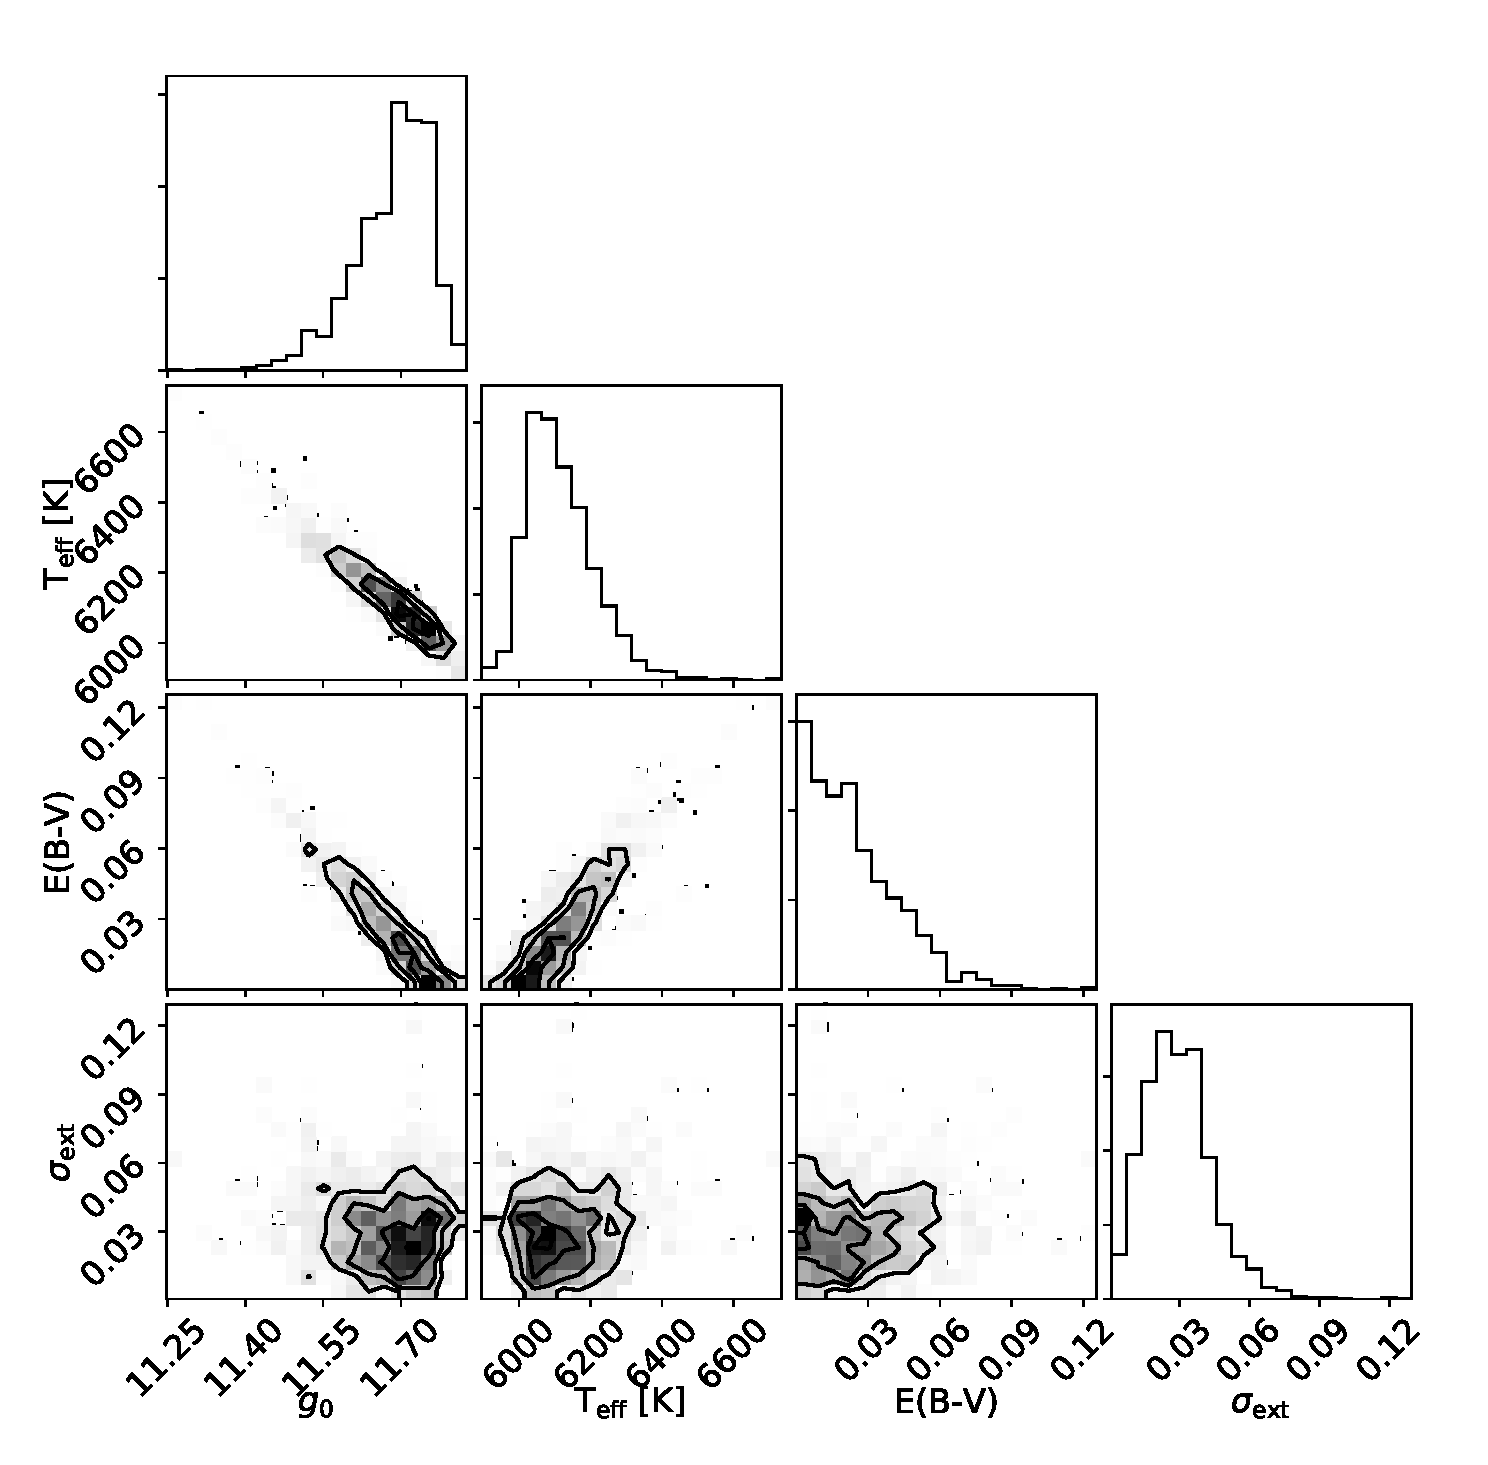
\includegraphics[scale=0.6]{7-images/SED_corner_J2349-32.eps}
    \caption{The posterior probability distribution of EBLM J2349$-$32 from photometric fitting. Over-plotted are the 68\%, 95\% and 99.7\% contours.}
    \label{methods:fig:SED_J2349-32}
\end{figure}







\section{Spectroscopic analysis}\label{methods:atmospheric_parameters}

\subsection{CORALIE - wavelet analysis}\label{methods:spectroscopy:wavelet}

The CORALIE spectra observations and reduction were carried out using the method outlined in Chapter \ref{chapter:wavelet} and \citet{2018A&A...612A.111G}, which is briefly describe here. I co-added the spectra and re-sample between 450-650\,nm with $2^{17}$ values. I calculated the wavelet coefficients $W_{i=4-14, k}$ (see Fig. \ref{fig:wavelet:filt} for visual justification of our choice of wavelet coefficients) and fit the same coefficients with model spectra in a Bayesian framework. I initiated 12 walkers and generate 10,000 draws as a burn-in phase. I sampled a further 10,000 draws to sample the PPDs for $T_{\rm eff}$, [Fe/H], $V\sin\,i$ and $\log g$. \citet{2018A&A...612A.111G} note that an [Fe/H] offset of -0.18\,dex which I correct for using Eqn. \ref{composition_correction}. I also note a  significant trend in $\log g$ with $T_{\rm eff}$ which I do not correct. The wavelet method for CORALIE spectra can determine $T_{\rm eff}$ to a precision of $85$\,K, [Fe/H] to a precision of 0.06\,dex and $V \sin i$ to a precision of 1.35\,km\,s$^{-1}$ for stars with $V \sin i$ $\geq$ 5\,km\,s$^{-1}$. However, measurements of $\log g$ are not reliable beyond confirming dwarf-like gravity ($\log g \approx 4.5$). Subsequently, I fitted the wings of the magnesium triplets with spectral synthesis by fixing $T_{\rm eff}$, [Fe/H] and $V\sin i$ and changing $\log g$ until an acceptable fit was found. 

\subsection{INT - synthesis}

INT observations of J1847$+$39 are unsuitable for wavelet analysis as only a small wavelength region around the H$\alpha$ line was observable with the H1800V grating.  The spectral synthesis technique was used to measure $T_{\rm eff}$ from the wings of the H$\alpha$ line and mean [Fe/H] from 11 unblended Fe lines around the H$\alpha$ line; I assumed an instrumental resolution of R$\approx$10,000. I determined a "good fit" by synthesising models which best match the spectra in shape and depth. This is assessed \textit{by-eye}.  I used the same model spectra used in Chapter \ref{chapter:wavelet} and Sect. \ref{methods:spectroscopy:wavelet}. There are no gravity sensitive lines visible in the INT spectra and so I assume $\log g = 4.44$. %Interpolating limb-darkening coefficients and evolutionary models requires an estimate of surface gravity, for which I estimate $\log g=4.44$ for J1847$+$39.


\section{First estimates for transit parameters}\label{methods:first_estimates}

Using the framework of \cite{2007ApJ...663..573B}, I obtained first order approximations to the ratio of semi-major axis, $a$, and the radius of the primary star, $R_{\star}$, using the width of the transit, $\Delta t_{\rm tr}$, 
%
\begin{equation}\label{approx_r_star}
\frac{R_{\star}}{a} \approx \pi \frac{\Delta t_{\rm tr}}{P},
\end{equation}
%
Assuming a circular orbit. The ratio of the radii, $k$, can be estimated
%
\begin{equation}\label{approx_k}
k = \frac{R_{2}}{R_{\star}} \approx \sqrt{\Delta m},
\end{equation}
%
where $R_2$ is the radius of the M-dwarf companion and $\Delta m$ is the depth of transit (in magnitudes). I used Eqns. \ref{approx_r_star} \& \ref{approx_k} to estimate starting positions for the orbital fit (Sect. \ref{method:orbital_fit}) using follow-up and K2 photometry.  



\section{Ephemerides}\label{ephem}

\begin{figure}
    \centering
    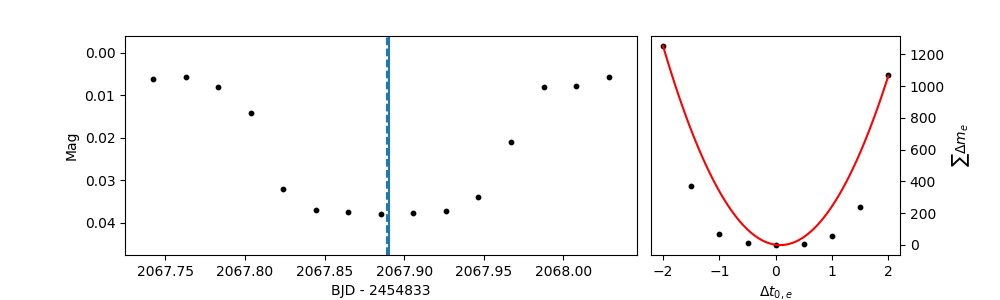
\includegraphics[scale=0.6]{7-images/1652-19_ephem.png}
    \caption{The minimum for the first transit of J1652$-$19 observed with K2 using the method of \protect\citet{1956BAN....12..327K}. (left panel) The first transit with predicted epoch (blue-solid) and calculated epoch (blue-dashed). (right panel) The sum of the residual magnitudes as a function of time from the predicted epoch with a fitted Gaussian model (red).}
    \label{method:fig:ephem1}
\end{figure}

\begin{figure}
    \centering
    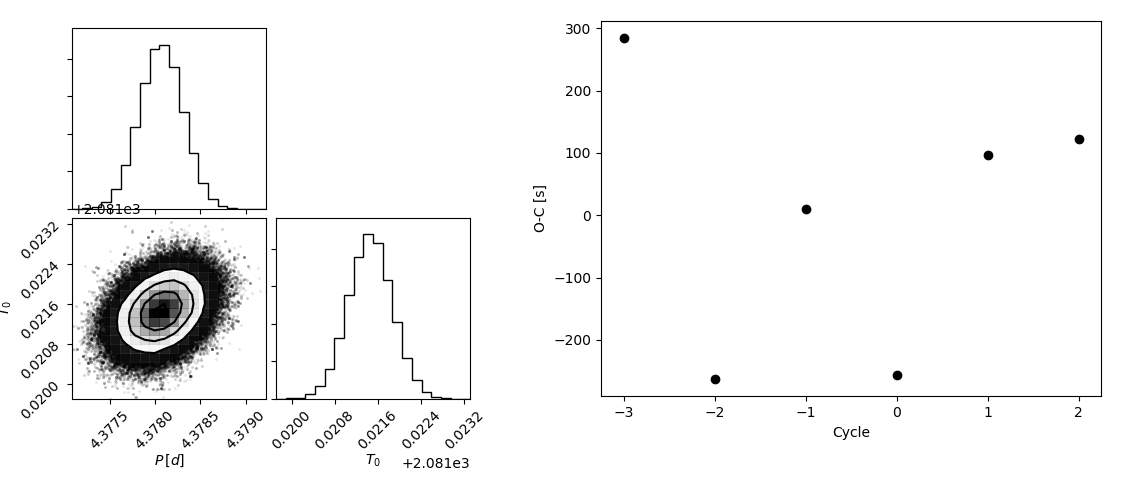
\includegraphics[scale=0.4]{7-images/1652-19_ephem_2.png}
    \caption{The corner plot for the period and epoch of J1652$-$19 (left). The residuals between predicted and observed epochs are also shown (right).}
    \label{method:fig:ephem2}
\end{figure}

 I used the method of \citet{1956BAN....12..327K} to accurately compute the epoch of minimum of each complete eclipse in the K2 photometry; WASP photometry was of insufficient quality to accurately measure the centre of individual transits. This method re-samples the time axis around a single transit and sums up the magnitude differences ($\sum m_e$) on each side of an arbitrary time, $t_{e}$. $t_{e}$ is advanced to the next time stamp where the process is repeated. The resulting values of $\sum m_e$ will form an inverted Gaussian which was fitted to determine the centre of the transit (minimum of $\sum m_e$) and the uncertainty (width of the Gaussian; Fig. \ref{method:fig:ephem1}).
 
 I minimised the correlation between subsequent transits and measured epochs by fitting a straight line in the form
 %
 \begin{equation}
     \rm epoch = P \times \rm cycle + T_0
 \end{equation}
 %
 where $P$ and $T_0$ are free parameters. I used \textsc{emcee} to initialise 100 walkers which were evolved for 10,000 steps. The first 5000 steps were discarded and the step with the highest log-likelihood was selected with uncertainties equal to the standard deviation of the PPD for each parameter (Fig. \ref{method:fig:ephem2}). I inspected the residuals between measured and found no evidence of transit-timing variations for any of the four EBLMs observed with K2.


\section{Out-of-transit photometry}\label{methods:photometric_variation}


I treated the out-of-transit photometry from WASP and K2 separately to determine if any period variations exist. In the following sections, I detail the methods used in each case.

\subsection{WASP photometry}

Each system has thousands of observations from the WASP survey which have been taken over many years. Consequently, it is possible to measure variations in the light-curve caused by spot coverage or tidal interactions. I used the method outlined in \citet{2011PASP..123..547M} to search the WASP photometry for frequencies attributed to rotational modulation. Each season of photometry is treated separately and in-transit data are excluded. I inspected the periodogram and false-alarm probabilities (FAP) for each system to assess the reliability of any detected periods. I also phase-fold the light-curve at the detected period to check for cases of ellipsoidal variation. The primary eclipses were masked in all cases along with potential secondary eclipses for J0055$-$00.

\subsection{K2}

\begin{figure}
    \centering
    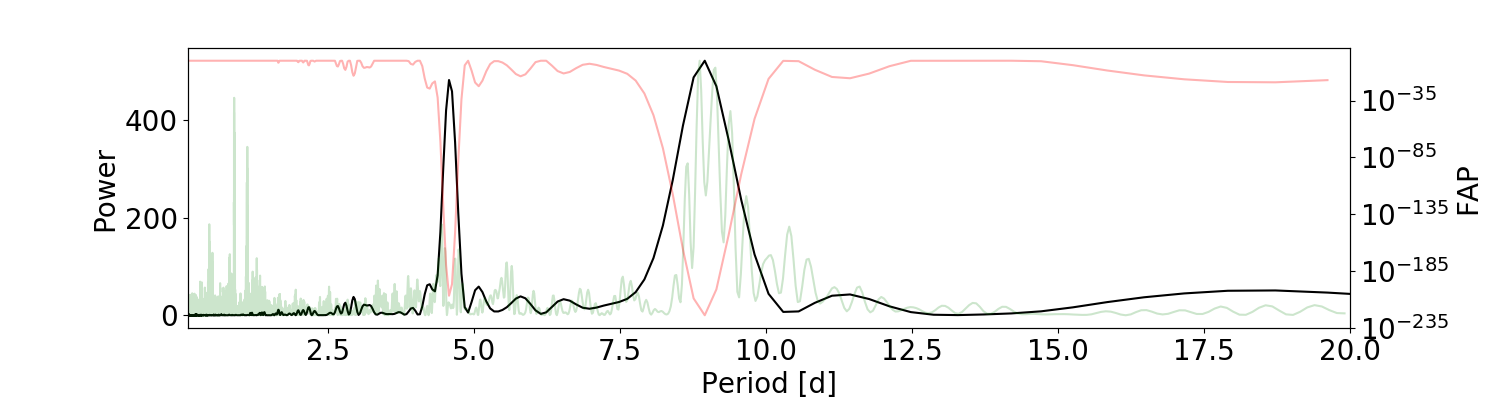
\includegraphics[scale=0.4]{7-images/J2217-04_period.png}
    \caption{The generalised Lomb-Scargle diagram J2217$-$04 for K2 photometry (black) with false-alarm probabilities (FAP; red). The Lomb-Scargle diagram of WASP photometry is also shown (green).  }
    \label{methods:fig:J2217-04_lomb}
\end{figure}

The quality of K2 photometry is such that I could visually search the generalised Lomb-Scargle periodigram to identify frequencies which match spot-like variation in the lightcurve. I used the \textsc{fasper} function provided within python package \textsc{k2sc} to calculate the Lomb-Scargle periodigram.  \textsc{fasper} uses a fast algorithm optimised for unevenly sampled data \citep{1989ApJ...338..277P} and reports the false-alarm probabilities attributed to significant periods. This is the probability of a signal being real with respect to the quality of the data. I analysed the raw lightcurve along with the periodigram to determine spot-induced variation and/or ellipsoidal variation. The primary eclipses were masked in all cases along with the secondary eclipses for J0055$-$00. The Lomb-Scargle periodigram for J1652$-$19 is shown Fig. \ref{methods:fig:J2217-04_lomb}, along with the rest of the EBLM sample in Appendix \ref{appendix:Lomb-Scargle}. 













\section{Orbital solution}\label{method:orbital_fit}

I determined the best-fitting orbital solution in different ways for EBLM systems with ground-based follow-up photometry (Table \ref{Observeration_table_ground}) and those observed with K2 (Table \ref{Observeration_table_K2}). This is due to the temporal nature of this work, in which I obtained data for the EBLMs with ground-based follow-up photometry much before those with K2 photometry. Subsequently, my method evolved to meet the requirements of the larger K2 data-sets. The following sections describe the similarities and differences between the two approaches. 

\subsection{EBLMs with ground-based follow-up photometry}

I fitted all follow-up  photometry (from SAAO, CTIO and HAO) and radial velocity measurements simultaneously to obtain the final orbital solution for each system. I performed a $\chi^2$ fit in a Bayesian framework to estimate the PPD of each parameter in the vector model. The vector model of parameters includes photometric zero-points for each $i^{th}$ light-curve -- $zp_{\rm i}$, $R_{\star}/a$, $k$, the impact parameter -- $b = a\cos(i)/R_{\star}$, $T_0$, $P$, the limb-darkening temperature -- $T_{\rm eff,ld}$, the semi-amplitude of radial velocity measurements for the primary star --$K_1$, the systematic radial velocity -- $\gamma$ and the change in systematic radial velocity with time --$d(\gamma)/dt$. The first estimate of $T_{\rm eff,ld}$ comes from the spectroscopic value of $T_{\rm eff}$ from Sect. \ref{methods:atmospheric_parameters}. First estimates of $R_{\star}/a$, $k$, $\rm T_0$ and $P$ were measured as described in Sec. \ref{methods:first_estimates} \&  \ref{ephem}. Instead of fitting the argument of the periastron ($\omega$) and the eccentricity ($e$), I chose to use the de-correlated parameters $f_c = \sqrt{e} \cos \omega$ and  $f_s = \sqrt{e} \sin \omega$ to improve the sampling efficiency at very low eccentricities, when $\omega$ is poorly constrained while maintaining a uniform prior on the value of eccentricity (see e.g. \citealt{2005AJ....129.1706F}). I also included a ``jitter'' term ($\sigma_J$) to account for spot activity which can introduce noise in to the radial velocity measurements \citep{2006ApJ...642..505F}. I used $T_{\rm eff,ld}$ to interpolate coefficients for the Claret limb-darkening law (provided with the python package \textsc{ellc}; \citealt{2016A26A...591A.111M}) using fixed values of [Fe/H] and $\log g$ from Sect. \ref{methods:atmospheric_parameters}. I used a Gaussian prior for $T_{\rm eff,ld}$ using the value of $T_{\rm eff}$ from Sect. \ref{methods:atmospheric_parameters} with a conservative uncertainty of 200\,K. Photometric and radial velocity models are synthesised using \textsc{ellc} assuming detached and spherical star-shapes.

I compare these models to data using a Bayesian framework with the likelihood function $\mathcal{L}(\textbf{d}|\textbf{m}) = \exp (-\chi^2/2)$, with
%
\begin{equation}\label{chi_squared}
\begin{split}
\chi^{2} = \sum_{i=1}^{N_{mag}} \frac{(m_{\rm i} - m_{\rm model})^2}{ \sigma_{m_{\rm i}}^2} &+ \sum_{i=1}^{N_{rv}} \frac{(rv_i - rv_{\rm model})^2}{\sigma_J^2 +  \sigma_{\rm rv_i}^2} \\ &+  \frac{(T_{\rm eff,ld} - T_{\rm eff})^2}{\sigma_{T_{\rm eff}}^2} .
\end{split}
\end{equation}
%
Here,  $m_{\rm i}$ and $rv_{\rm i}$ represent the $i^{th}$ measurement of magnitude and radial velocity with standard errors $\sigma_{m_{\rm i}}$ and $\sigma_{\rm rv_i}$,  respectively. I initiated 50 walkers and generated 50,000 draws, after an initial burn-in phase of 50,000 draws. I initially selected the model with the highest value of $\mathcal{L}(\textbf{d}|\textbf{m})$ from the PPD to extract the best-fitting model parameters. For J2308$-$46 and J1847$+$39 I found these values to be up to 2-$\sigma$ away from the median value of each parameters PPD, and so I chose the measurements to be the median value from each parameters PPD instead. The uncertainties were calculated from the largest difference between the median and the $16^{th}$/ $84^{th}$ percentile of the cumulative PPD for each parameter from the second chain.


\subsubsection{Rossiter-McLaughlin}

I obtained radial velocity measurements of J0218$-$31 during transit that display variations caused by the Rossiter-McLaughlin effect. The orbital fit for this system required two more de-correlated parameters,  $\sqrt{V \cos i} \sin \lambda$ and $\sqrt{V \sin i} \cos \lambda$, where $\lambda$ is sky-projected angle between the orbital and stellar rotation angular momentum vectors.

\subsubsection{Star shapes}

 \begin{figure}[htb]
  \centering
  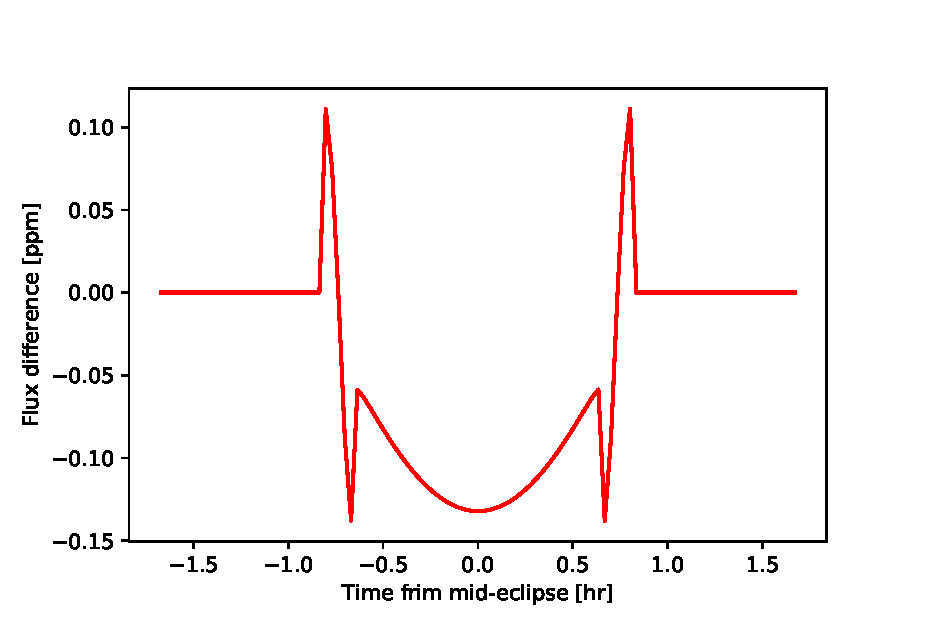
\includegraphics[scale=1]{7-images/model_difference.eps}
  \caption {The difference between the spherical model and Roche model  of J2308$-$46 using \textsc{ellc}.}
  \label{methods:fig:model_diff}
\end{figure}
 
 % I found ellipsoidal variations in the WASP photometry of EBLM J2308$-$46 which required the use of Roche geometry to estimate the initial  transit parameters from the WASP photometry. The follow-up photometry of EBLM J2308$-$46 was fitted using a spherical star shape  with the assumption that there is only a small amount of out-of-eclipse photometry, which was detrended. 
 
 I assume stars are well separated and thus spherical. A caveat is that the spherical volume of the star will not be the same as the volume of the triaxial ellipsoid used to approximate its shape with \textsc{ellc}. I assessed the magnitude of this problem by comparing the models for J2308$-$46 where both stars are described by spheres to those where both stars are described using Roche models (Fig. \ref{methods:fig:model_diff}).  I found a maximum difference of $\approx 0.1\, \rm ppm$ which is far below the white-noise level (a few thousand ppm) and so I did not attempt to correct for this. %The final orbital solution for all EBLMs assumes detached and spherical star-shapes and does not use Roche geometry.
 
 \subsubsection{Primary eclipses}
 
 I modelled the primary eclipses for all EBLMs (excluding  assuming J0055$-$00) assuming that the luminosity from the M-dwarf is negligible compared to the light from the primary star. Including light from the M-dwarf will have the effect of diluting the primary transit depth. Assessing whether a correction is needed for this effect requires some foreshadowing of the results (Chapter \ref{chapter:results}). For the largest M-dwarf in my sample, J1436$-$13 ($M_2 \approx 0.5\,M_\odot$, $k \approx 0.28$, $\log g_2 \approx 5$) I estimate a surface temperature $\approx$3700\,K by using MESA stellar models (\citealt{2016ApJ...823..102C}; \citealt{2016ApJS..222....8D}). I convolved \textsc{phoenix} model spectra \citep{2013A&A...553A...6H} for each companion with the K2 band-pass to estimate the M-dwarf's flux contribution  $\sim$0.47\% of the total luminosity. By inspecting synthetic lightcurves from \textsc{ellc}, I estimated a dilution of the primary transit depth by $< 500$\,ppm; this is below the photometric precision of the ground-based light-curves and so I do not apply a transit-depth correction for these systems. The EBLMs observed with K2 have smaller values of $k$ and so the expected flux contribution from the M-dwarf is smaller. However, the photometric precision is much higher and so the potential for introducing a bias increases. For J1652$-$19 ($M \approx 0.25\,M_\odot$, $k \approx 0.15$, $\log g_2 \approx 5$), the primary transit depth is modified by $<30$\,ppm when accounting for the luminosity of the M-dwarf; the rms scatter of the K2 lightcurves is between 200-1000\,ppm. 1652$-$19 is fairly representative of the K2 EBLMs in this work and so I do not apply any corrections for the primary transit depths of these systems.  For J0055$-$00, including a non-zero surface-brightness ratio in the model automatically modified the models primary eclipse depth. This is fortunate since J0055$-$00 has the best photometric precision of the K2 sample and would have been most susceptible to a bias of the transit depth from the M-dwarfs luminosity. EBLMs with early-type M-dwarfs, cooler primary stars and high-quality lightcurves will require due diligence to ensure there is no bias introduced by neglecting the flux contribution from the M-dwarf. 

 
 
 
 \subsection{EBLMs observed with K2}
 
 The K2 data sets are more sizeable than single transits obtained from ground-based telescopes. This resulted in a significantly larger computation time to create photometric models and increased the time taken to determine the orbital solution. I decided to stray away from the claret 4-parameter limb darkening law in favour of the power-2 law \citep{1997A&A...327..199H} as recommended by \citet{2017AJ....154..111M} for its performance in the remit of 2-parameter limb-darkening laws and for cooler stars. The power-2 law has an analytical approximation (Maxted \& Gill, 2018. in prep) which significantly decreases the time taken to calculate models (see Sect. \ref{discussion:qpower2} for timing tests and Appendix X). The law consists of two parameters ($\alpha$ \& $c$) and has the form,
%
\begin{equation}
I(\mu) = 1 - c(1 - \mu^{-\alpha}). 
\end{equation}
%
The parameters $\alpha$ \& $c$ are strongly correlated. Instead, I fitted the decorrelated parameters
%
\begin{eqnarray}
h_1 &= 1 - c(1 - 2^{-\alpha}) \\
h_2 &= c2^{-\alpha} \\
\end{eqnarray}
%
with inverse transformations
%
\begin{eqnarray}
c &= 1 - h_1 + h_2 \\
\alpha &= \log_2(c/h_2).
\end{eqnarray}
%
The parameter $h_1$ measures the specific intensity relative to the centre of the disk in the region on the stellar disk ($r = \sqrt{1 − 1/2} \approx 86.6\%$) and $h_2$ measures the drop in relative intensity from the same distance and the limb. Look-up tables are provided by \citet{2018A&A...616A..39M} using synthetic 3D LTE spectra from the Stagger-grid calculated by \citet{2015A&A...573A..90M}. I decided against interpolating values of $h_1$ and $h_2$ for a given $T_{\rm eff,ld}$ as it was computationally expensive. I fitted $h_1$ and $h_2$ using Gaussian priors centred at the values interpolated from \citet{2018A&A...616A..39M} using atmospheric parameters from Sect. \ref{methods:atmospheric_parameters} and width of 0.011 and 0.045 respectively \citep{2018A&A...616A..39M}. In the following sections I describe the fast transit model (\textsc{qpower2}) used for K2 datasets along with the red-noise model to account for out-of-transit variations.

\subsubsection{\textsc{qpower2}}

The theory of Keplerian orbits is largely covered in Chapter \ref{chapter:theory}. Determining photometric and radial velocity modesl hinges on the calculation of the true anomaly, $\nu$, from the other five Keplerian elements. The \textsc{qpower2} model uses the \textsc{batman} transit model \citep{2015PASP..127.1161K} as a template to solve Keplers equations for $\nu$. Instead of using Newton-Raphson iteration to solve for the eccentric anomaly, $E$, I used the algorithm from \citet{1997CeMDA..66..309F} which avoids transcendental function evaluations. This carries a small maximum error on the order of $10^{-16}$. I also used the analytical expression for the time of periastron passage prior to a given time of eclipse ($t_c$) which assumes an inclination of $90^\circ$. The difference in flux caused by this approximation is approximately 50\,ppm in ingress and egress for an inclination of $87^\circ$ \citep{2016A26A...591A.111M}. The sky-projected orbital separation in units of stellar radii, $z$, is then calculated using Eqn. \ref{sky_projected_seperation} along with radial velocities from Eqn. \ref{radial_velocity}. 

The normalised flux in an eclipse, $F$, depends on the area of the primary star covered by the M-dwarf, $Z$, and the specific intensity, $I_\lambda (r)$,
%
\begin{equation}
    F = 1 - \int_Z I_\lambda (r) dA ,
\end{equation}
%
where $I_\lambda (r) = 1 - c + c(1 - r^2)^{\alpha / 2}$. Evaluating this integral requires use of hypergeometric functions which is computationally expensive. Instead, I derived an approximation to this integral
by replacing $I_\lambda (r)$ by a truncated Taylor series --
%
\begin{equation}
    I_\lambda (r)) \approx  I_\lambda (r_0) + (r - r_0)I'_\lambda (r_0) + \frac{1}{2}(r - r_0)^2 I''_\lambda (r_0)\,...,
\end{equation}
%
where primed symbols denote derivatives with respect to r. How this Taylor expansion is evaluated depends on the projected sky-seperation between the primary star and M-dwarf companion, $z$. For the case where $z \leq 1 - p$ the disk of the M-dwarf lies completely within the disk of the primary star. By using $r_0 = z$ as the reference point for the Taylor series expansion and numerous approximations, the flux drop can be approximated by
%
\begin{equation}
    F \approx 1 - I_0 \pi k^2 \left[c_o = \frac{1}{4} k^2 c_2 - \frac{1}{8} \alpha c k^2 s^{\alpha/2 - 1} \right],
\end{equation}
%
where
\begin{eqnarray}
c_0 &= 1 - c + c s^{\alpha/2} \\
c_2 &= \frac{1}{2} \alpha c s^{\alpha /2 - 2}\left( (\alpha - a) k^2 - a \right),
\end{eqnarray}
and $s = 1 - z^2$.

For ingress and egress phases ($1 - p < z < 1 + p$) the integral is evaluated in two regions separated by the chord defined by the intersections between the two limbs. This
chord is at a distance $d = (z^2 - k^2 + 1) / 2z$ from the origin. Care must be taken in choosing the reference point $r_0$ in the Taylor expansion because $I'(r)_\lambda \rightarrow \infty $ for $r \rightarrow 1$. To avoid this problem and to ensure continuity with the light curve at other phases I choose $r_0 = r_a = (z - p + d)/2$ to evaluate the integral over the region between the chord and the limb of the planet, and $r_0 = r_b = (1 + d) / 2$ for the region between the chord and the limb of the star.  I then find that the lightcurve at these phases can be approximated by 
%
\begin{equation}
    F \approx 1 - I_0 ( J_1 - J_2 + K_1 - K_2),
\end{equation}
%
where$J_1$,  $J_2$,  $K_1$ and  $K_2$ are coefficients  arising from the Taylor expansion of $I_\lambda (z)$ (Maxted \& Gill, 2018. in prep). A python implementation of this algorithm is given in Appendix X.

\begin{landscape}
 \begin{figure}
  \centering
  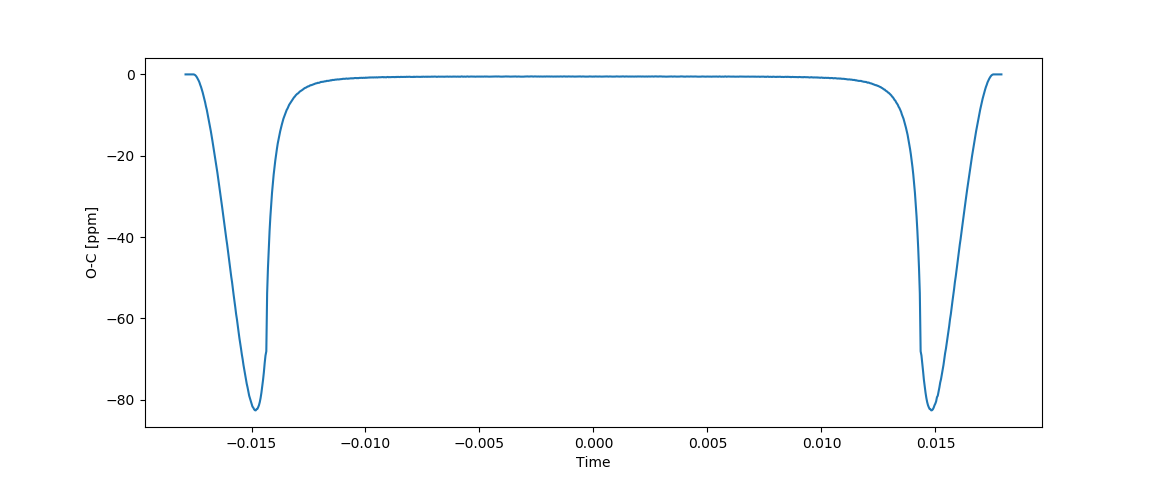
\includegraphics[width=0.9\linewidth,keepaspectratio]{7-images/qpower_ellc_test.png}
  \caption{The difference between \textsc{ellc} and the \textsc{qpower2} algorithm for a circularised system with $R_\star = 0.2$ and $k=0.2$. }
  \label{method:fig:qpower2_ellc}
 \end{figure}
\end{landscape}

I compared the accuracy of the the \textsc{qpower2} algorithm with \textsc{ellc} for a system with $R_\star / a = 0.2$ and $k = 0.2$ (Fig. \ref{method:fig:qpower2_ellc}). From this figure it can be seen that the \textsc{qpower2} algorithm reproduces light curves for the power-2 limb-darkening law accurate to better than 0.008\% for these parameters. For J0055$-$00, I required an accurate prescription for the secondary eclipse. I assumed that the M-dwarf companion is uniformly illuminated which permits an analytical expression for the secondary eclipse. I use the formalism provided within the \textsc{batman} package to calculate the secondary eclipse transit shape for a given value of $z$ and surface brightness ratio, $S$. I was careful to adjust the depth of the primary eclipse appropriately for a given value of $S$. For J0055$-$00, $S$ was added to the model vector of the orbital solution and fitted with a uniform prior between 0--0.2.



\subsubsection{Red noise model}\label{methods:rednoise}

\begin{figure}
    \centering
    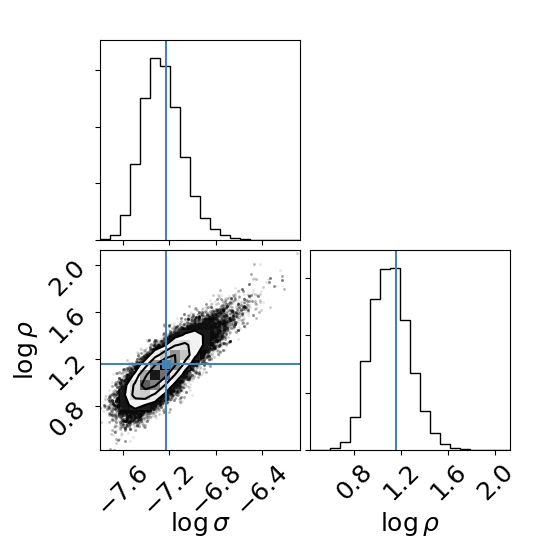
\includegraphics[width=0.5\textwidth]{7-images/220196587_GP_parameters.png}
    \caption{The correlation between $\log \sigma$ and $\log \rho$ for J0055$-$00.}
    \label{method:fig:celerite_corrolation}
\end{figure}

Photometric variations in the K2 lightcurve required a suitable red-noise model to complement \textsc{qpower2}. I used the \textsc{celerite} package \citep{2017AJ....154..220F} and the following kernel with the default value of $\epsilon=0.01$ to approximate the Mat\'{e}rn-3/2 covariance function: 
%
\[ k(\tau) = \sigma^2\,\left[
  \left(1+1/\epsilon\right)\,e^{-(1-\epsilon)\sqrt{3}\,\tau/\rho}
  \left(1-1/\epsilon\right)\,e^{-(1+\epsilon)\sqrt{3}\,\tau/\rho} \right]. \]
%
 Here, $\tau$ is the time difference between two observations and $\rho$ is a parameter that controls the time scale over which observational errors are correlated and $\sigma$ controls the amplitude of such variations. This introduced two detrending parameters to the model vector: $\log \sigma$ and $\log \rho$.  These two parameters are well constrained for all lightcurves (eg. see Fig. \ref{method:fig:celerite_corrolation}) and I used uniform priors between $-20$ and $20$ for each parameter.



\section{Masses, radii and age}\label{methods:eblmmass}

Breaking the degeneracy between the mass of the primary star -- $M_{\star}$, the M-dwarf companion -- $M_2$, and the age of the system -- $\tau$, is non-trivial. One approach by \citet{2009ApJ...693.1920H} uses Kepler's equation to estimate the density of the primary,
%
\begin{equation}\label{density}
\rho_{\star} = \frac{3 \pi}{GP^2} \left( \frac{a}{R_{\star}} \right)^3 - \frac{3M_2}{4 \pi R_{\star}^3}
\end{equation}
%
and then combine it with measurements of $T_{\rm eff}$ and [Fe/H] to interpolate between stellar models for $M_{\star}$ and $\tau$. Typically, this is repeated with a better estimate of $M_{\star}$ until the solution converges iteratively. Another approach uses empirical mass and radius calibrations (\citealt{2011MNRAS.417.2166S}; \citealt{2013AN....334....4T}) to obtain $M_{\star}$ and $R_{\star}$.  These are combined with $k$ and eqn. \ref{density} to obtain $M_2$ and $R_2$. A third approach by \citet{2013A&A...549A..18T} mixes the two methods while fitting orbital parameters. The mass function \citep{Hilditch2001} can be expressed in terms of radial velocity parameters,
%
\begin{equation}\label{mass_function}
f(m)  =  \frac{(M_2 \sin i)^3}{(M_{\star} + M_2)^2} =  (1-e^2)^{\frac{3}{2}} \frac{P K^3}{2 \pi G},
\end{equation}
%
where $G$ is the gravitational constant. The middle and right part of Eqn. \ref{mass_function} can be equated and solved numerically for $M_2$ assuming an initial guess of $M_{\star}$ from empirical calibrations. Stellar models are interpolated to give a new estimate of $M_{\star}$. The new value of $M_{\star}$ can be used to iteratively solve Eqn. \ref{mass_function} and generate better estimates of $M_{\star}$ and $M_2$ until a solution is converged upon. A final method relies on three assumptions: (1) the circularisation timescale ($\tau_{\rm circ}$) is much shorter than $\tau$, (2) the rotation is synchronised ($\tau \gg \tau_{\rm sync})$ and (3) that rotational and orbital inclination are the same. With these assumptions it is possible to directly calculate the mass and radius of both components without dependency on stellar models (see Eqns. 14-17 of \citealt{2007ApJ...663..573B}).

To measure the mass and age of the primary star I combined the atmospheric parameters (Sect. \ref{methods:atmospheric_parameters}) and the best fitting orbital solution (Sect. \ref{method:orbital_fit}) and interpolate between evolutionary models computed with the \textsc{garstec} stellar evolution code \citep{2008Ap&SS.316...99W}. To achieve this, I make no assumptions regarding orbital circularisation or synchronisation. I use da modified version of the open-source code \textsc{bagemass} \citep{2015A&A...575A..36M} tailored exclusively for EBLM systems (\textsc{eblmmass}). \textsc{eblmmass} uses the jump parameters of age, primary mass ($M_{\star}$), the initial iron abundance in dex $\rm [Fe/H]_i$, $\rm M_2$ and the full-width half maximum of the transit $w$. The vector of  observed parameters is given by $\textbf{d} = (f(m),\,\rm T_{\rm eff}, \, \rm \log L_{\star}, \, \rm [Fe/H]_s, R_{\star}/a, w )$ where $\log L_{\star}$ is the luminosity of the primary star and $\rm [Fe/H]_s$ is the surface metal abundance in dex and $w$ is the transit width. The model parameters are $\textbf{m} = (M_{\star}, M_2, \tau, \rm [Fe/H]_i, w )$. $\rm [Fe/H]_s$ differs from the initial abundance ($\rm [Fe/H]_i$) due to diffusion and mixing processes throughout stellar evolution. The \textsc{garstec} evolutionary models used here are the same as the ones used in \textsc{bagemass}. \textsc{garstec} uses the FreeEOS\footnote{http://freeeos.sourceforge.net} equation of state \citep{2003ApJ...588..862C} and standard mixing length theory for convection \citep{1990sse..book.....K}. The mixing length parameter used to calculate the default model grid is $\alpha_{\rm MLT} = 1.78$. With this value of $\alpha_{\rm MLT}$ \textsc{garstec} reproduces the observed properties of the present day Sun assuming that the composition is that given by \citet{1998SSRv...85..161G}, the overall initial solar metallicity is $Z_{\sun} = 0.01826$, and the initial solar helium abundance is $Y_{\sun} = 0.26646$. These are slightly different to the value in \citet{2013PhRvD..87d3001S} because I have included additional mixing below the convective zone in order reduce the effect of gravitational settling and so to better match the properties of metal-poor stars. Due to the effects of microscopic diffusion, the initial solar composition corresponds to an initial iron abundance [Fe/H]$_{\rm i} = +0.06$ dex. The stellar model grid covers the mass range $0.6 M_{\odot}$ to $2.0 M_{\odot}$ in steps of $0.02 M_{\odot}$. The grid of initial metallicity values covers the range [Fe/H]$_i$ = $-0.75$ dex to $-0.05$ dex in steps of $0.1$ dex and the range [Fe/H]$_i$ = $-0.05$ to +$0.55$ in $0.05$ dex steps. 

To obtain $M_2$ from $f(m)$, $M_{\star}$ and $P$, I needed to know inclination from the transit light-curve. Degeneracies between $i$, $R_{\star}/a$ and $k$ are such that I chose to fit the full-width half maximum of the transit,
%
\begin{equation}\label{fwhm_transit}
w = \frac{R_{\star}}{a} \frac{\sqrt{1-b^2}}{\pi} ,
\end{equation}
%
instead of the inclination. I implemented a Gaussian prior on $\rm [Fe/H]_s$ from spectroscopy and use a uniform priors for age, $M_{\star}$ and $M_2$. I ran a burn-in chain of 100,000 draws before drawing 50,000 draws to sample the PPD for $M_{\star}$, $M_2$ and $\tau$. The number of post-burn-in draws matches that of the orbital fit so I can measure the M-dwarf temperature for J0055$-$00 (Sect. \ref{method:M_dwarf_temp}) and assess the fractional radius and temperature residuals (Sect. \ref{discuss:inflation} \& \ref{discuss:J0055-00T2}).


I used an up-to-date constant from IAU resolution B3 \citep{2016AJ....152...41P} to calculate $a$ from $P$, $M_{\star}$ and $M_2$,
%
\begin{equation}
a = 4.208278 \times P^{\frac{2}{3}} (M_{\star} + M_2)^{\frac{1}{3}}.
\end{equation}
%
This can then be combined with $R_{\star}/a$ and $k$ to calculate the PPD for $R_{\star}$ and $R_2$. I selected the the median value of each parameters PPD as our measurements, with uncertainty equal to the largest difference between the median and the $16^{th}$ and $84^{th}$ percentile of the cumulative PPD for each parameter from the second chain.




\section{M-dwarf temperature for J0055$-$00}\label{method:M_dwarf_temp}

The K2 photometry of J0055$-$00 has secondary eclipses from which $S$, and thus $T_{\rm eff, 2}$, can be determined . Converting $S$ to a PPD for $T_{\rm eff, 2}$ demands a comparison of spectral energy distributions for the primary star and the M-dwarf which have been convolved with the K2 band-pass. I chose to use the \textsc{pheonix} stellar models \citep{2013A&A...553A...6H}.  For each draw in the PPDs from \textsc{eblmmass} and the orbital solution, the procedure was as follows:

\begin{enumerate}
    \item Random values of $T_{\rm eff}$, [Fe/H] and $\log g$ were generated from normal distributions using the mean as the measurements from Table.\ref{EBLMs_atmos} and the respective uncertainties as widths. These were used to interpolate a \textsc{pheonix} model spectra for the primary star. 
    
    \item The same value of [Fe/H] with the corresponding draw for $\log g_2$ was used to continually interpolate spectra for a value of $T_{\rm 2}$ that matched the light ratio predicted in the K2 band-pass from the corresponding draw of $S$ and $k$ (until $\Delta S \leq 10^{-4}$).
\end{enumerate}
The PPD for $T_{\rm eff}$ was fitted with a Gaussian from which the measurement of $T_{\rm eff}$ was taken to be the peak, with uncertainty equal to the standard deviation.




















\iffalse
\subsection{Image alignment}\label{image_alignment}

Measuring the transit of an eclipsing binary system requires simultaneous observations of the system and a few reliable field stars. The pixel-to-pixel variations of optical CCDs require each star to remain on, or very close to the same pixel for subsequent observations to avoid systematic trends in aperture photometry. Most instruments employ the use of a \textit{guide star} observed either through a separate finder telescope or the main telescope. The pixel-to-pixel shifts from subsequent observations of guide star are translated into corrections for the telescope control system. These measures keep target stars on the same CCD position within a couple of pixels depending on the instrument. Precise time series photometry still requires the pixel offsets to be calculated from image-to-image to adjust the aperture position and provide useful information for detrending the measured fluxes.

I aligned CCD observations from SAAO 1-m and Kepler/K2 using the Fourier alignment method. A reference image is convolved with the sample image which is reversed in both x and y dimension. The convolved image is then summed along the x and y dimension. The collapsed axes of the convolved image are similar to the cross-correlation functions obtained in Sect. X and were fitted with Gaussian function (Eqn. Y). The peak of the Gaussian was chosen to be the offset ($\Delta x$ or $\Delta Y$) with $\sigma$ as the uncertainty. The python code can be seen in Sect. A. 

A caveat of this method is its sensitivity to dead, hot or unresponsive pixels. The presence of these features creates a strong signal at $\Delta x = 0$ and $\Delta y = 0$, hoodwinking this method. A solution is to choose parts of the CCD chip which does not enclose such features.  

\subsection{Flux and magnitude calculations}

Extracting the flux of a star requires the use of an \textit{aperture} which encloses the target star. The SAAO 1-m observations were periodically checked to ensure the focus of the telescope yielded a near-spherical point-spread function for the target star. For these observations I chose a circular aperture. The radial profile from the centre of each star was inspected to find the radius which enclosed most of the power from the star (Fig. Y). This was chosen to be the radius of the aperture. The flux $F_i$ at time $t_i$ for the target star was calculated by summing all the pixel values which fall entirely within the aperture. Pixels partially within the aperture were weighted depending on the fraction of area that falls within the aperture. The arbitrary magnitude can then be calculated,
\begin{equation}
m_i = -2.5 \log_{10} (F_i) .
\end{equation}
The uncertainty in in $m_i$ ($\sigma_{m_i}$) can be estimated from the sky background flux, $\sigma_{\rm sky}$.  The sky background flux is calculated by summing the the counts  from an annulus with inner and outer radius greater than the aperture used to calculate $F_i$ to sample the sky flux around the target star.  The error in magnitude is essentially the difference in magnitude associated with $F_i$ counts and $F_i  - \sigma_{\rm sky}$ counts,
\begin{eqnarray}
\sigma_{m_i} &= -2.5 \log_{10} \left( \frac{F_i - \sigma_{\rm sky}}{F_i} \right) = -2.5 \log_{10} \left(1 -  \frac{\sigma_{\rm sky}}{F_i} \right) .
\end{eqnarray}A caveat to this type of photometry  is that ground based observation will follow the star through a variety of different air-masses as the target rises and eventually sets. The airmass is usually quantified as $\sec Z$, where $Z$  is the angular zenith distance. Thus $m_i$ is typically correlated with $\sec Z$ which is unhelpful. Excluding this effect requires flux measurements of a second star on the CCD image. Trends in measured flux for the target star will equally effect the second star assuming they are sufficiently close  that they both have the same value of $\sec Z$. This is also the case for other environmental factor such as CCD drifts and sporadic increases in atmospheric seeing. It is then possible to calculate the \textit{differential magnitude},
\begin{equation}
\Delta m_i = -2.5 \log_{10} \left( \frac{F_i}{F_2} \right)
\end{equation}
Where $F_2$ is the flux from star 2. The aperture for star 2 should be similar to star 1 and star 2 should be chosen to be as close to the target star as possible, be non-varying with time and be of similar apparent magnitude.

Photometric observations from the Kepler/K2 mission are above the atmosphere and do not suffer from atmospheric effects. The gain and band-pass is well characterised allowing $F_i$ to be calculated in absolute terms, and thus $m_i$ can be calculated as the Kepler magnitude. 

\subsection{Quality assurance}

The uncertainty, $\sigma$, from Sect. \ref{image_alignment} is a useful proxy for image quality. During observations with intermittent clouds, or when alignment fails, $\sigma$ increases beyond normal values and can be used to identify images which may lead to bad measurements of $F_i$. The uncertainty in magnitude measurements, $\sigma_{m_i}$, is a useful tell of quality. If clouds drift into the field-of-view then $\sigma_{\rm sky} \approx F_i$. Inspection of $\sigma_{\rm sky}$ relative $F_i$ is a good diagnostic for the reliability of $F_i$ when observations are made in poor weather. The transit light-curves were inspected \textit{by-eye} as a final check to ensure quality measurements.
\fi